\graphicspath{{literature_study/fig/}}

\chapter{Literature Study}
\label{chap:literature_study}

%%%%%%%%%%%%%%%%%%%%%%%%%%%%%%%%%%%%%%%%%%%%%%%%%%%%
\section{Soil moisture sensor}
Capacitive soil moisture sensors have two electrodes that form a planar capacitor with soil acting as the dielectric material as shown in figure \ref{fig:capacitor}. 

\begin{figure}[!h]
    \centering
    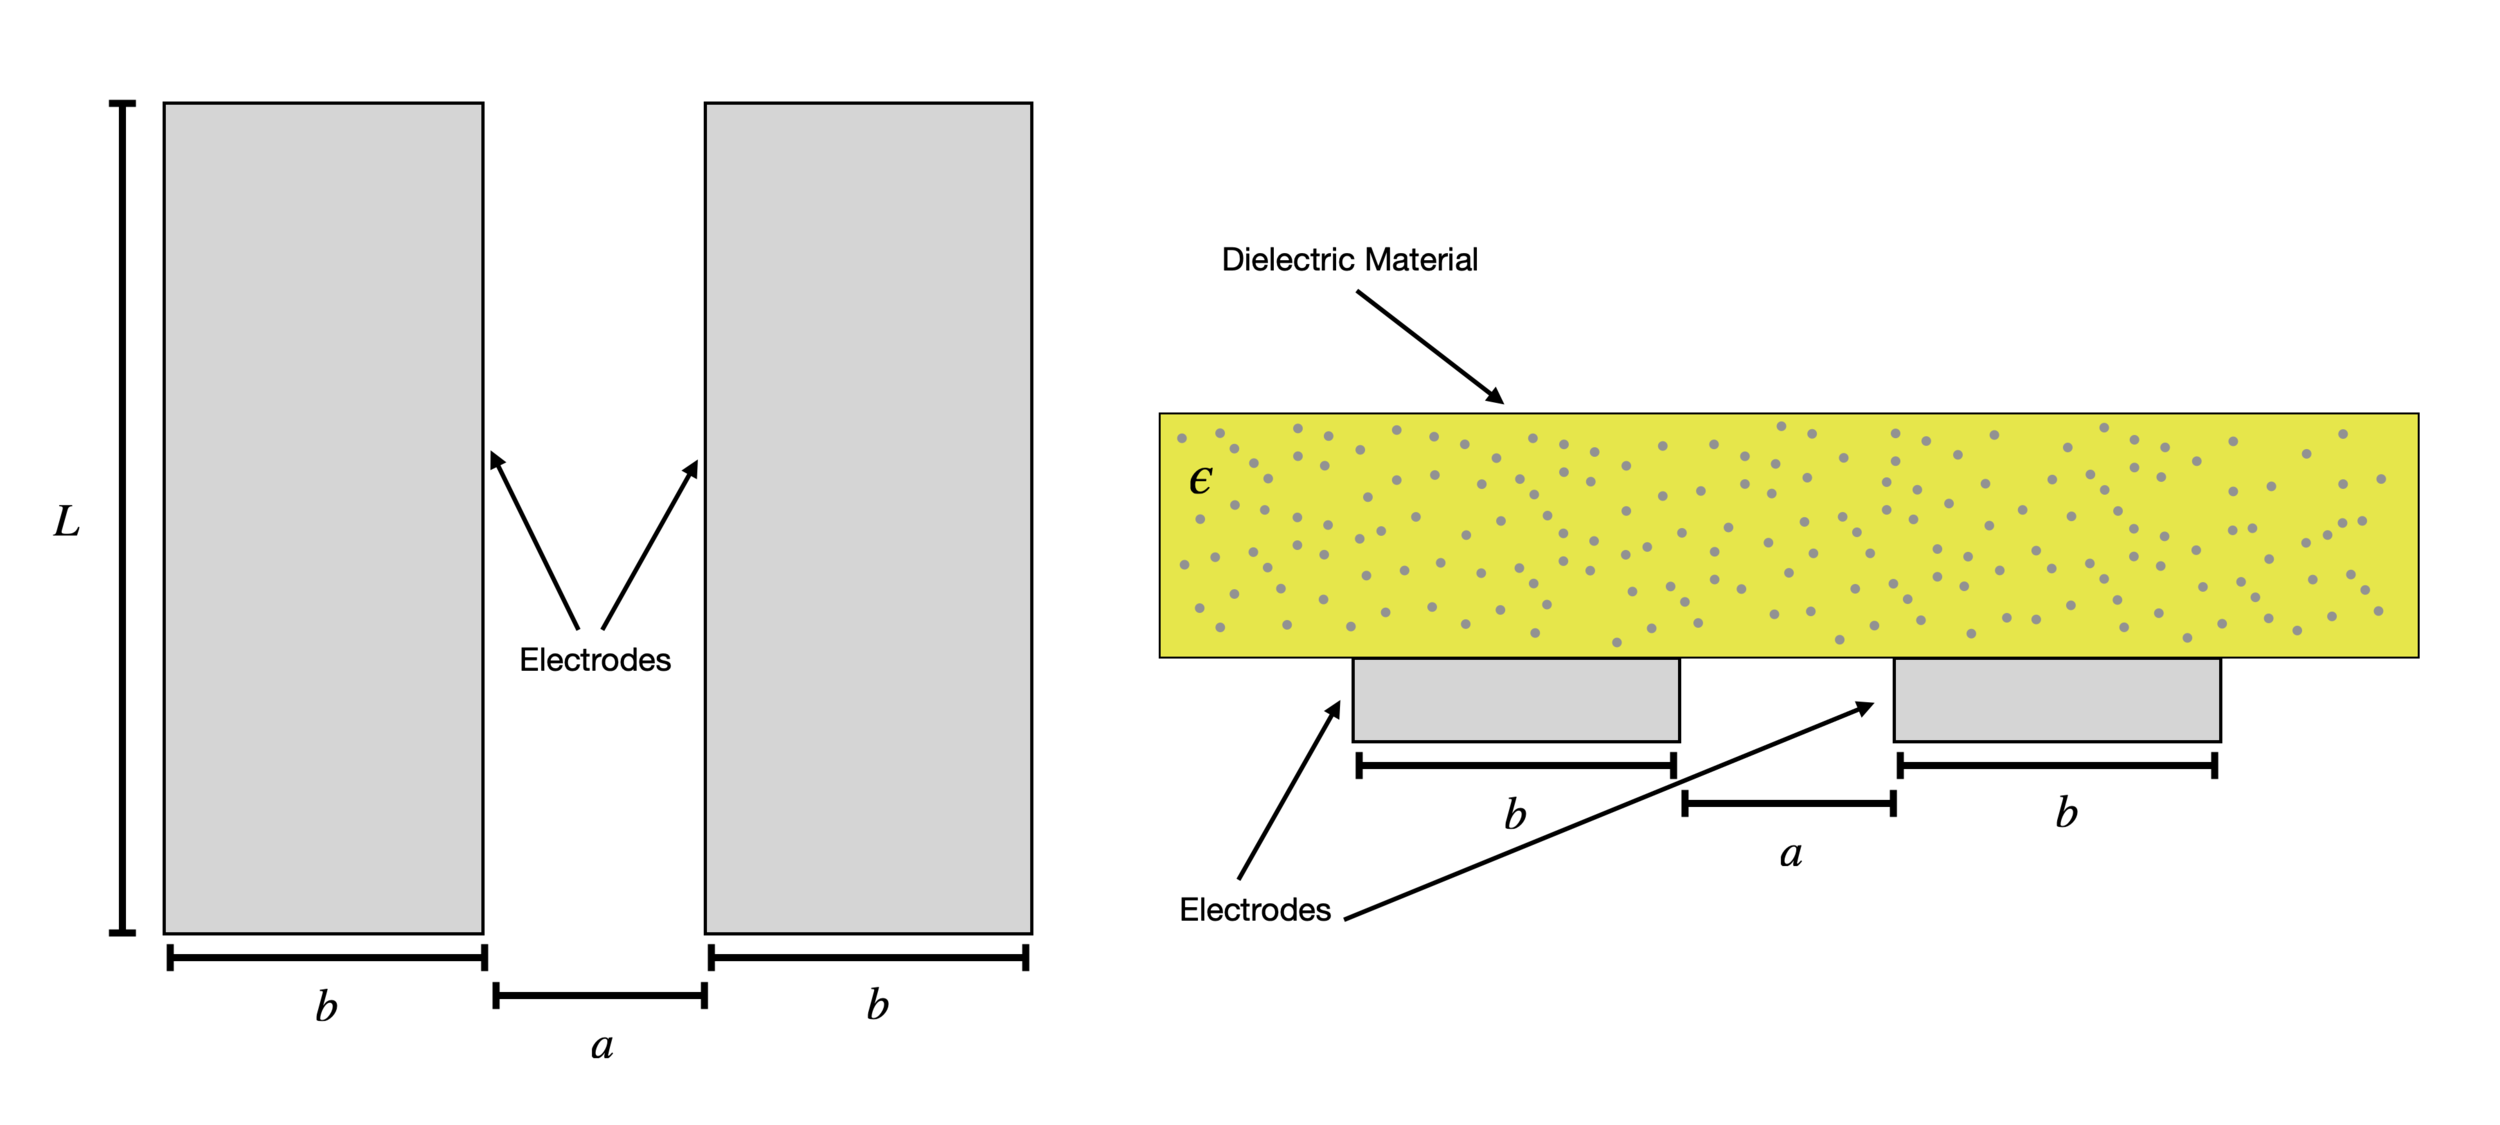
\includegraphics[width= 0.9\linewidth]{coplanar_capacitor_drawing.png}
    \caption{Planar capacitor \cite{moisture_sensor_img}}
    \label{fig:capacitor}
\end{figure}

The percentage of water will change the dielectric constant of the soil and therefore the capacitance. The sensor uses a timer to output a PWM voltage proportional to the capacitance of the soil. \cite{moisture_sensor_img}

%%%%%%%%%%%%%%%%%%%%%%%%%%%%%%%%%%%%%%%%%%%%%%%%%%%%
\section{UV light sensor}
Ultraviolet light has a wavelength range of 100 to 400 nm and can be measured using a photodiode or photo-resistor. These produce either a current or resistance that is dependant on UV radiation. The sensor outputs a voltage proportional to this current or resistance. \cite{UV_sensor}

%%%%%%%%%%%%%%%%%%%%%%%%%%%%%%%%%%%%%%%%%%%%%%%%%%%%
\section{Battery options}
Do research on Li-ion and lead acid. pros, cons and charging methods

